\subsection{Function discriminant analysis, FDA}

The FDA, also known as function discriminant analysis, is an
intermediate solution between analytical solutions in the linear case
such as Fisher discriminant and non-linear ones such as artificial
neural networks. The aim of the FDA method is to solve relatively
simple or partially non-linear problems. The user must provide a
desired function with adjustable parameters via TMVA option
string. The formula must be in format accepted by ROOT TFormula. FDA
algorithm then fits parameters to it with the requirement that the
function value for the signal is as close as possible to 1 and for
background as close as possible to 0.

The advantage of this method is the simplicity and transparency of the
expression that is used for discrimination. However its performance
depends heavily on the user defined discriminator function. This is
certainly a disadvantage in problems where phase space dependent
nonlinear correlations exist. FDA should reproduce the performance of
any linear discriminant analysis method. In non-linear domain the
discriminator must include more complicated non-linear terms.
 
\begin{figure}[h]
 \begin{minipage}{8.5cm}
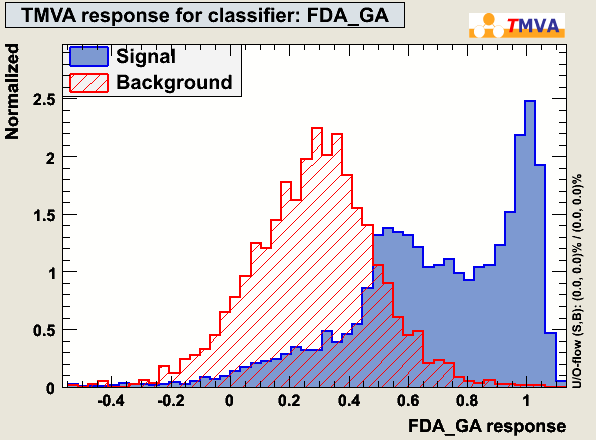
\includegraphics[width=1.0\textwidth]{images/pkMva_FDA_GA.png}
\end{minipage}
 \hfill
\begin{minipage}{8.5cm}
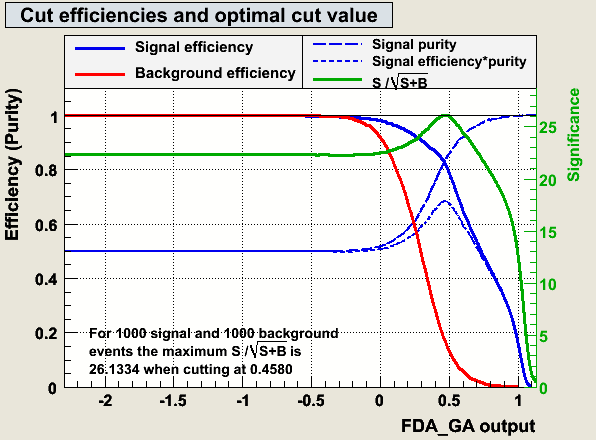
\includegraphics[width=1.0\textwidth]{images/pkMvaEffs_FDA_GA.png}
\end{minipage}
\caption{Left: mvaFDA using genetic algorighm (GA). Right: FDA GA}
\label{fig:pkMvaFDAGA}
%\label{fig:pkMvaEffsFDAGA}
\end{figure}


\begin{figure}[h]
 \begin{minipage}{8.5cm}
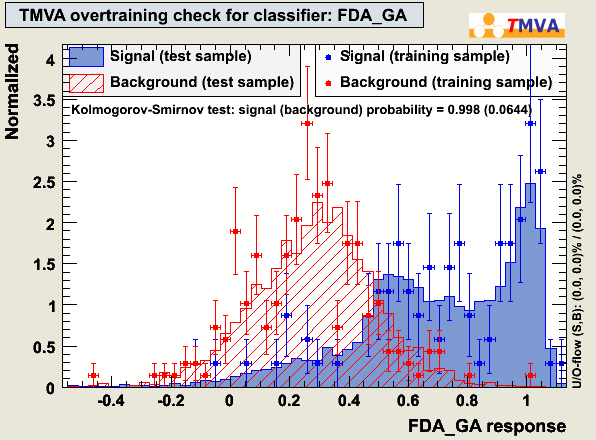
\includegraphics[width=1.0\textwidth]{images/pkOvertrain_FDA_GA.png}
\end{minipage}
 \hfill
\begin{minipage}{8.5cm}
FDA GA
\end{minipage}

\label{fig:pkOvertrainFDAGA}
\end{figure}


\subsection{k-nearest neighbour method, kNN}

The multidimensional k-nearest neighbour, also known as k-NN, method
is conceptually fairly similar to the PDERS method. The k-NN is an
adaptive algorithm which searches for a fixed number of adjacent
events. These events define the volume for the metric, i.e. the
distance, that is used. The simplest metric is the Euclidean one. The
$k$ events with the smallest values of $R$ are called
\emph{k-nearest neighbours}.

 The number of variables in feature space and the number of
neighbours investigated, depend on the particular data at
hand. Generally larger values of investigated neighbours reduce the
effect of noise in the classification but it also makes the boundaries
between classes less distinct. The k-NN classifier performance
surpasses that of parametric learning methods when the boundary
separating signal from background contains irregular features.

Internally k-NN uses so called k-dimensional trees, or kd-trees, for
sorting the training events. The kd-tree is a data structure for
organizing the points in a k-dimensional space. The TMVA
implementation of kd-trees is reasonably fast one.

It should be noted that TMVA developers do not recommend using this
classifier for problems with more than about 10 variables. In general
the larger the data set the more this algorithm probes the small scale
differences in signal and background.

\begin{figure}[h]
 \begin{minipage}{8.5cm}
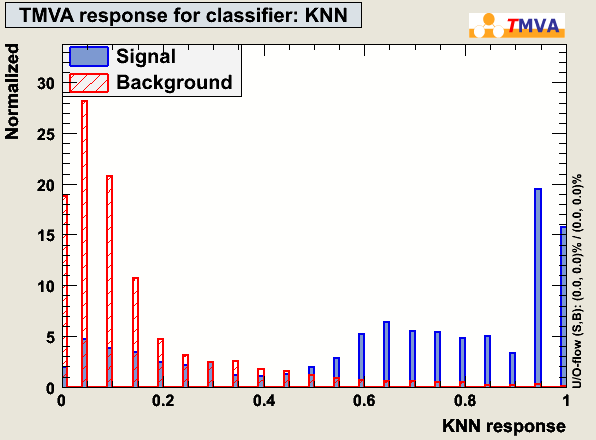
\includegraphics[width=1.0\textwidth]{images/pkMva_KNN.png}
\end{minipage}
 \hfill
\begin{minipage}{8.5cm}
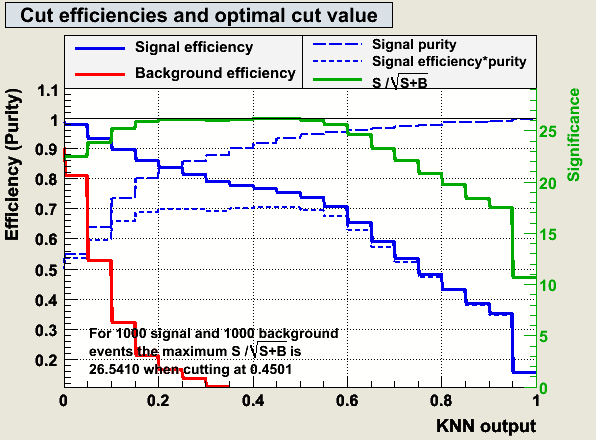
\includegraphics[width=1.0\textwidth]{images/pkMvaEffs_KNN.png}
\end{minipage}
\caption{Left: MVAKNN. Right: KNN effs}
\label{fig:pkMvaKNN}
%\label{fig:pkMvaEffsKNN}
\end{figure}


\begin{figure}[h]
 \begin{minipage}{8.5cm}
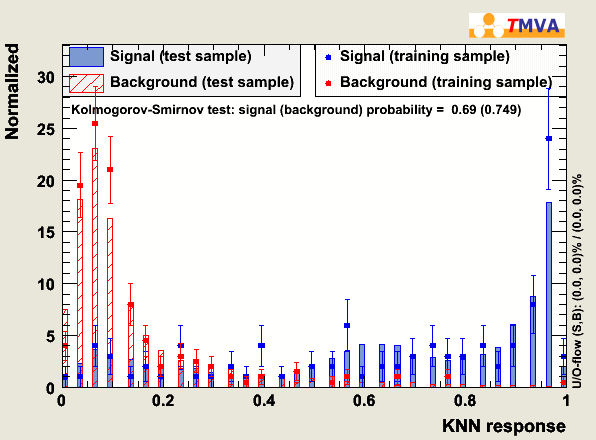
\includegraphics[width=1.0\textwidth]{images/pkOvertrain_KNN.png}
\end{minipage}
 \hfill
\begin{minipage}{8.5cm}
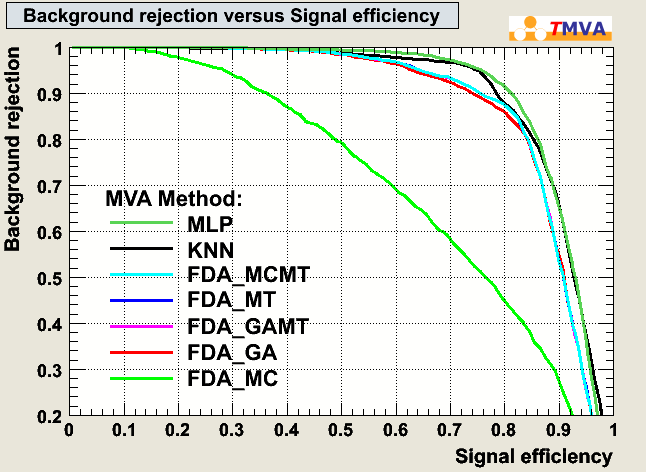
\includegraphics[width=1.0\textwidth]{images/pkRejBvsS.png}
\end{minipage}
\caption{Left: KNN. Right: ROC curve (MLP added as a benchmark)}
\label{fig:pkOvertrainKNN}
%\label{fig:pkRejBvsS}
\end{figure}

\clearpage
